



\title{La Galaxia Espiral Roja UGC11680: La Evidencia de Apagado en formaci\'{o}n estelar ``Dentro-Fuera''}
\author{
        Jeffrey E. B\'{a}rcenas Mosqueda \\
                Instituto de Astronom\'{i}a\\
        Universidad Nacional Aut\'{o}noma de M\'{e}xico\\
        jbarcenas@astro.unam.mx
}
\date{\today}

\documentclass[12pt]{article}

\usepackage{graphicx}  
\usepackage{balance}    
\usepackage[utf8]{inputenc}
\usepackage[T1]{fontenc}
\usepackage[square]{natbib}
\usepackage{amsmath}
\usepackage{amsfonts}
\usepackage{amssymb}
\usepackage{caption}
\usepackage{subcaption}
\usepackage{wrapfig}
\usepackage{lettrine}
\usepackage{morefloats}
\usepackage{color}
\usepackage{natbib}
\usepackage{hyperref}
\usepackage{aas_macros}

%\newcommand\araa{ARA\&A}%
%\newcommand\aaps{A\&AS}%
%\newcommand{\aap}{A\&A}

\citestyle{aa}


\begin{document}
\maketitle



\section{Introducción}

En el catálogo del muestreo \textbf{CALIFA} (Calar Alto Legacy Integral Field Area (\cite{sanchez2012}) hay una galaxia espiral roja peculiar llamada UGC11680. Esta galaxia está a un  \textsl{redshift} de $z \sim 0.026198$ (esto es a una distancia cosmológica de $\sim$ 113 Mpc)  clasificada como una SBb Seyfert 2 (\cite{blazquez2007}) y que esta situada en el diagrama Color-Magnitud en la zona conocida como ``secuencia roja'' normalmente habitada por grandes galaxias elípticas, donde sabemos que por dicho color, ya no forman estrellas y que por lo tanto la ubica dentro de las galaxias que sufrieron un apagado en su formacion estelar y que sin embargo conservan su morfología espiral. De esta manera, Dado que su morfología es conservada, es poco probable que procesos de fusión o interacción fuerte, sean los responsables del apagado de UGC11680, aunque en el analisis de esta galaxia, no supondremos ni descartaremos ninguna hipótesis \textsl{apriori}, por lo que nuestros resultados son exclusivamente fenomenológicos. 

\noindent Los procesos físicos que dan lugar a este apagado, (conocido en la literatura como ``quenching'') están bajo debate y se encuentran dentro de los temas sin consenso  en la astronomía extragaláctica actual. Por un lado, algunos autores señalan procesos externos que  ``desnudan'' a la galaxia de gas fresco para la formación de estrellas nuevas  (\cite{salim2007}, \cite{noeske2007},\cite{peng2010},\cite{dimatteo2005}) otros autores señalan factores internos que apagan la formación estelar \cite{martin2007}, \cite{nandra2007}, \cite{schawinski2007}).

\section{Análisis de Datos}

Antes de Analizar que sucedio con UGC11680, descartamos la contaminación por polvo, ya que este podria enrojecer la galaxia y hacerla cambiar de color en el óptico (Sin embargo esto es poco probable ya que la galaxia se encuentra de cara y en general es conocido que el polvo a esa inclinación es de poca importancia). El valor encontrado fue de de $A_v \sim 1 $ mag  aunque alto, no es capaz de cambiar el color de UGC11680. Ya sin la presencia de polvo, analizamos la historia de formación estelar (SFH) de UGC11680, a través sus poblaciones estelares por medio de datos de la espectroscopía de campo integral. Para esto, utilizamos el pipeline \textbf{PIPE3D} y el código \textbf{FIT3D} (\url{http://www.astroscu.unam.mx/~sfsanchez/FIT3D/index.html}), diseñada para el análisis de cubos de datos resultado de este tipo de técnica. De este novedoso análisis obtenemos imágenes y espectros  espacialmente resueltos y del resultado del proceso de datos, analizamos los mapas de historia de formación estelar \cite{cid2013_1}, y que arrojaron una clara evidencia del \textsl{quenching}
de la  galaxia de prueba en un tiempo dado, (ver figura \ref{ugc11680}).


\begin{figure}[ht]
  \centering
  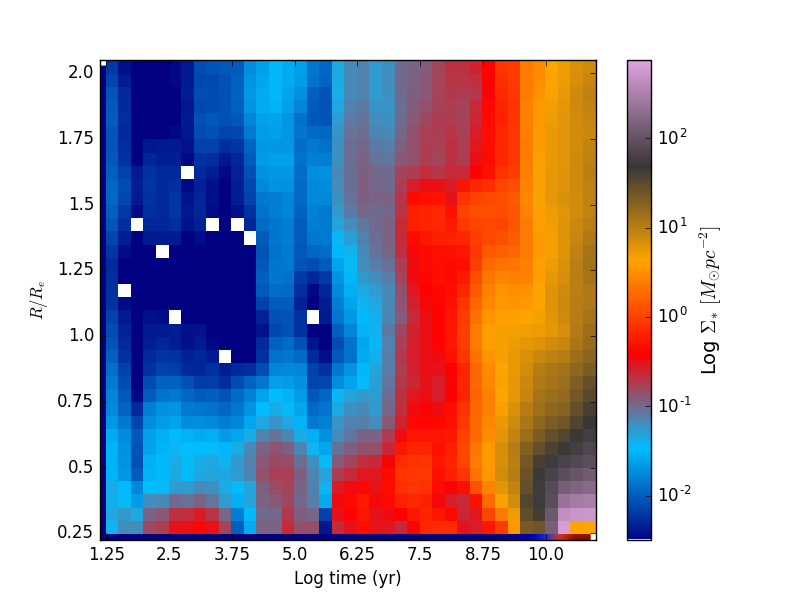
\includegraphics[width=5in]{/media/jeffrey/KINGSTON/Tesis_marzo/sfh_map_ugc11680.png}
  \caption[spectra]
   {\small \textsl{El resultado principal para nuestro analisis: el mapa de formación estelar en tiempo y radio,es decir, la $SFH(t,R)$. El radio esta sobre el eje $y$, normalizado con su radio efectivo  $R_e$ y el tiempo es el eje $x$ en escala logarítmica.El gradiente de color es densidad de masa estelar superficial  $\Sigma_{*}$. Nótese el cambio repentino de color en el centro de UGC11680  (como una ``mordida''  en la zona central, de un color oscuro a un ligero tono rojizo) En alrededor de $\sim$ 8.5 log yr.}}
\label{ugc11680}
\end{figure}

\begin{figure}
  \centering
    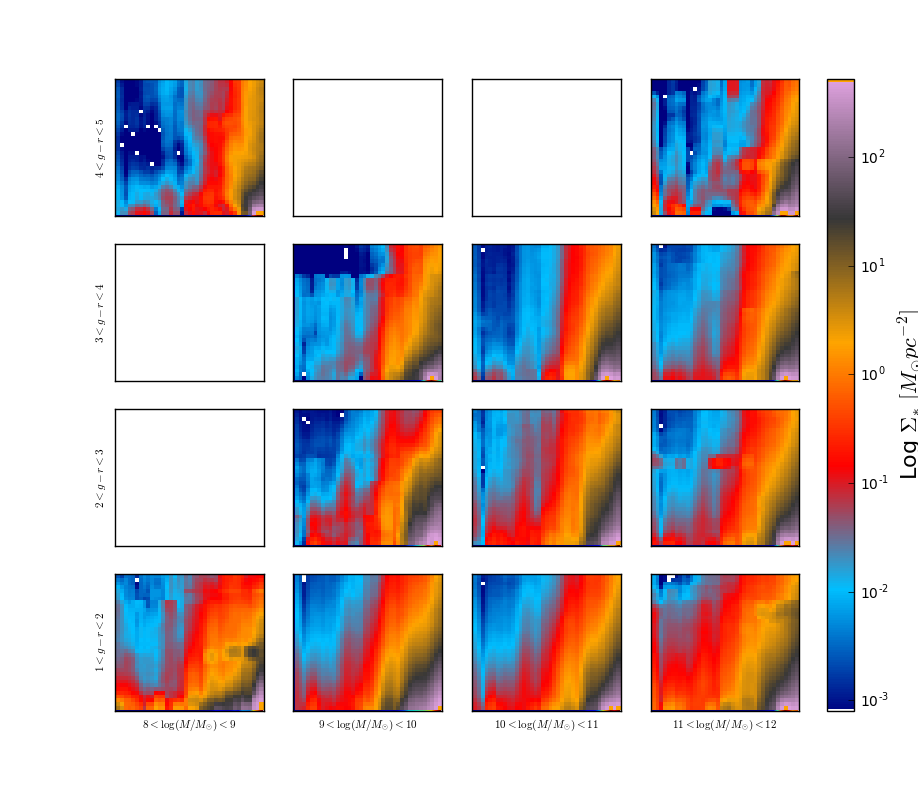
\includegraphics[scale=0.6]{cmd_sfh.png}
  \caption{Diagrama Color-Masa  para las $SFH(t,R)$ pertencientes a su intervalo correspondiente.
           Cada $SFH(t,R)$ de la muestra de  \textbf{CALIFA} individual fue promediado con todos los de su categoría,
           por lo que cada una de ellas muestra un promedio para el intervalo de color-masa correspondiente. En la esquina superior izquierda, esta el mapa de UGC11680, por comparación.La cantidad de galaxias para cada categoria. Las escalas temporales y radiales son las mismas que se dieron para mapas de galaxias individuales.Nótese el ensamblaje más grande para galaxias más masivas, además de el lento ensamblaje de las galaxias más ligeras, además del apagado de UG11680, mas notorio debido al escalamiento.}
  \label{CMD}
\end{figure}

Finalmente, la Historia de formación estelar de UGC11680  es comparada con la del resto de las 574 galaxias  de la muestra de \textbf{CALIFA}, separadas y clasificadas en sus valores color-masa usando la medida $\chi^2_{\nu}$ \footnote{Dado que hablamos de una medida reducida, es decir, una $\chi^2$ dividida por el número de grados de libertad $\nu$ definimos ``parecido '' a el número mas cercano a 1,y por lo tanto una $\chi^2_{\nu} =1 $ denotaría un parecido exacto} y encontrando que la historia de formacion estelar de UGC11680 es una combinacion en ``parecido''  con el grupo de 24 AGNs de la muestra de \textbf{CALIFA} espacialmente resueltos y de aquellas galaxias que se encuentran en el  del diagrama color-masa y que esta en la figura \ref{CMD} que se supone es un espacio de transición entre la secuencia roja y la nube azul (ver figura \ref{chiagns}).

\begin{figure}[ht]
  \centering
  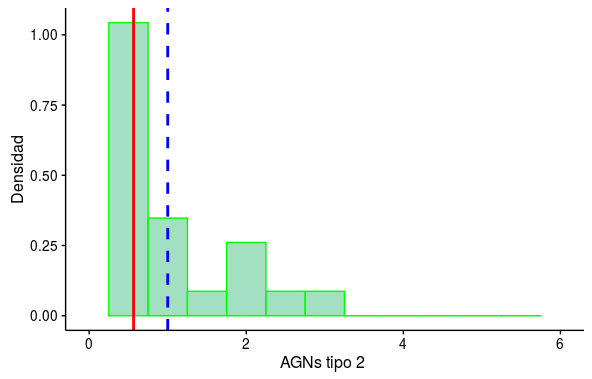
\includegraphics[width=5in]{/media/jeffrey/KINGSTON/Tesis_marzo/chi_agns.png}
  \caption[spectra]
   {\small \textsl{La distribución de probabilidad $\chi^2$ para los 24 AGNs tipo 2 en la muestra de  \textbf{CALIFA}. La linea negra punteada es el valor $\chi^2$ de UGC11680 con respecto al promedio ponderado de las  historias de formación estelar de estos AGNs. Siendo UGC11680 un AGN también, se dejo fuera de este promedio, para no contaminarla busqueda de parecido. Notese entonces que el valor de  $\chi^2$ de UGC11680 con respecto a la media de todos los AGNs es casi idéntica, lo que implica una historia de formación estelar común}.}
\label{chiagns}
\end{figure}


%\begin{figure}[ht]
 % \centering
 % \includegraphics[width=5in]{figure_4.png}
  %\caption[chicm]
   %{The $\chi^2$ probability distribution for the Color-Mass bins. The dashed black line is the UGC11680 $\chi^2$ with respect to each averaged bin}
%\label{chicm}
%\end{figure}


 Este valle verde, nos ofrece pistas sobre la naturaleza y duración de las transiciones para  galaxias de la nube azul a la secuencia roja. Esta transición
debe ocurrir en escalas de tiempo relativamente rápidas, de lo contrario habría una acumulación de galaxias en esa zona, en lugar de una
acumulación en la secuencia de roja, tal como se observa (\cite{arnouts2007}, \cite{martin2007}. las galaxias en el valle verde tienen por tanto, detalles escenciales para la evolución de galaxias,(\cite{bell2004}. \cite{faber2007}, \cite{martin2007}, \cite{schiminovich2007},\cite{wyder2007}, \cite{mendez2011}; \cite{goncalves2012}, \cite{schawinski2014}). Para nuestro caso, parece ser que capturamos a una galaxia que recientemente ($\sim$ Myrs) salio del valle y se ubicó en la secuencia roja.
%\begin{figure}[ht]
 % \centering
  %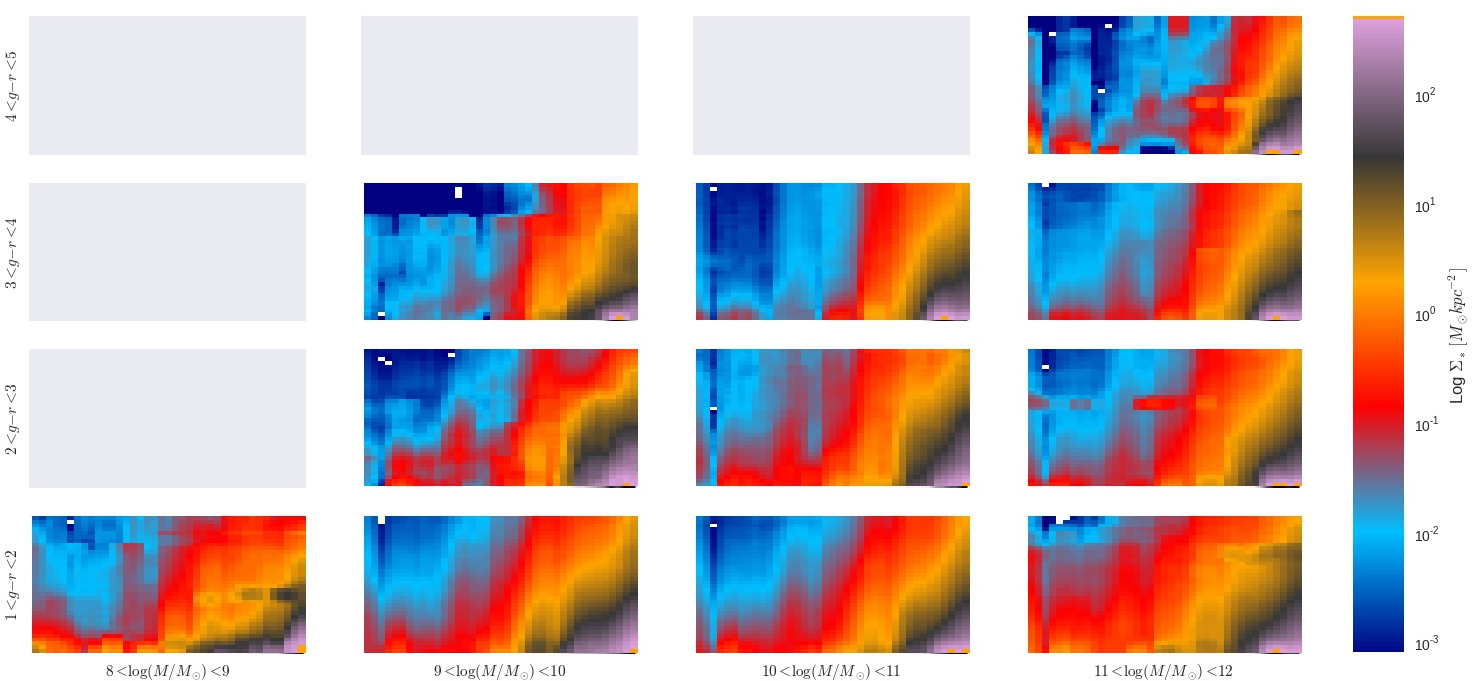
\includegraphics[width=3in]{figure_13.png}
  %\caption[spectra]
   %{Diagrama Color-masa de la muestra de \textbf{Califa}. Cada caja es el promedio ponderado de las  $SFH(t,R)$  de cada galaxia,dado el color y la masa correspondiente. El gradiente de color denota la densidad de masa superficial  $\Sigma_{*}$. En esta figura es mas evidente el crecimiento ``Dentro-fuera'' conforme la masa crece. Notese también que el ensamblaje de masa es mas rápido para galaxias más pesadas y rojas, mientras que es mas lento para galaxias ligeras y azules, así como un crecimiento ``fuera-dentro'' para ellas.}
%\label{cm1}
%\end{figure}



\section{Conclusiones y Resultados}

Con los resultados obtenidos, podemos dar un esbozo de la evolución de UGC11680: UGC11680 ensambló su masa de dentro hacia afuera, y en un momento de su historia de formación, encendió el AGN y algún proceso apago su formación estelar de dentro hacia afuera,(esto es más evidente en en el mapa $SFH(t,R)$) y que a pesar de todo, la influencia del AGN no es suficiente para el apagado total, ya que como lo muestra el mapa, la galaxia sigue formando estrellas, pero no a una tasa que permita observar un cambio de color evidente, lo que implica su posición dentro de la secuencia roja. Dado que los AGNs y sus galaxias huéspedes pertenecen a diferentes tipos de galaxias (elípticas y espirales) La distribución $\chi^2_{\nu}$ muestra que la media en genaral y el valor  $\chi^2_{\nu}$ de UGC11680 en particular, pertenecen a una historia de formación estelar en común, no importando en que galaxia huesped se encuentren. Esto nos da indicios de que la retroalimentación del AGN es de alguna manera (Aún no sabemos como)  un actor fundamental en la evolución de galaxias que lo contienen.





\bibliographystyle{apj}
\bibliography{/media/jeffrey/KINGSTON/Tesis_marzo/Bibliografia/referencias}

\end{document}
This is never printed
